\section{约束资格}
\label{sec:kkt-cq}

定理~\ref{thm:kkt-tangent-necessary}是关于切锥的，而能算的是线性化锥。两者之间差一个包含关系。本节研究：约束函数在一点满足什么条件，线性化就没有引入虚假方向，也就是切锥等于线性化锥？这类只涉及约束函数、不涉及目标的条件称为\term{约束资格}（constraint qualification）。

约束资格和凸性是两回事。约束$x^2\leq0$是凸函数，问题也可以是凸的，但它的线性化在原点失效。反过来，圆周这样的非凸集合，线性化却是准确的。约束资格检查的是约束函数在这一点的一阶信息够不够用，和目标函数是否凸没有关系。

\subsection{线性无关约束资格}
\label{sec:kkt-licq}

先看线性化为什么可能准确。在圆周的$(1,0)$处，沿切线走一步$(1,t)$会离开圆周，但偏离只有$t$的二阶小量，沿圆的法向拉回去一点，就回到圆周上。拉回动作所需的修正量比$t$小得多，放大看不出来，所以切线方向是真实可行的。

这个拉回动作要能实施，需要约束的梯度在拉回的方向上足够“有劲”，也就是各约束可以被独立地修正。这就是下面的条件。

\begin{definition}[线性无关约束资格]
\label{def:kkt-licq}
设$\bar{\bm{x}}\in\bm{C}$。若向量组
\begin{equation}
 \{\nabla h_j(\bar{\bm{x}}):j=1,\ldots,p\}\cup\{\nabla g_i(\bar{\bm{x}}):i\in A(\bar{\bm{x}})\}
 \label{eq:kkt-licq}
\end{equation}
线性无关，就称$\bar{\bm{x}}$满足\term{线性无关约束资格}（linear independence constraint qualification，LICQ）。
\end{definition}

图~\ref{fig:kkt-licq-representation}(a)是预算例的角点，梯度$(1,1)$和$(0,-1)$线性无关，LICQ成立。图(c)是上一节的尖点，两个活动梯度共线，LICQ不成立。圆周上$\nabla h=(2x_1,2x_2)$处处非零，单个非零向量线性无关，LICQ处处成立。约束$x^2\leq0$在原点的梯度为零，LICQ不成立。

\begin{BookInlineFigure}
  \centering
  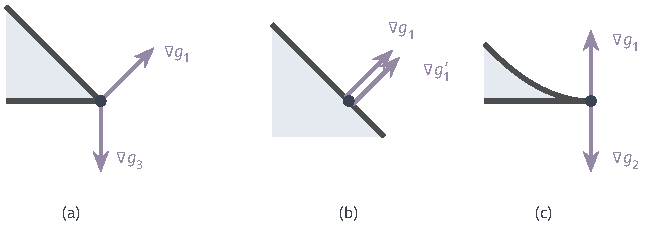
\includegraphics[width=110.3mm]{figures/05-optimization/06-constrained-optimization/tikz/kkt-licq-representation/figure.pdf}
  \caption{活动约束的梯度是否线性无关（紫色箭头）。(a)角点处两条梯度线性无关，LICQ成立。(b)同一条约束写两次，可行集不变，但两个梯度相同（为看清而错开绘制），LICQ不成立。(c)尖点处两个梯度方向相反，LICQ不成立。}
  \label{fig:kkt-licq-representation}
\end{BookInlineFigure}

下面的引理把“拉回”写成隐函数定理的一次应用，它产生一条真正可行的曲线。第~\ref{sec:kkt-second-order}节的二阶必要条件还要用这条曲线。隐函数定理说：方程关于待解变量的Jacobian可逆时，方程在局部确定唯一的连续可微解，详见\BookChapterRef{chap:implicit-inverse-functions}{卷二第22章“隐函数与反函数”}。

\begin{lemma}[沿线性化方向的可行曲线]
\label{lem:kkt-feasible-curve}
设约束函数在$\bar{\bm{x}}\in\bm{C}$附近连续可微，$\bm{d}\in\bm{F}(\bar{\bm{x}})$。设$W\subseteq A(\bar{\bm{x}})$满足：$i\in W$时$\langle\nabla g_i(\bar{\bm{x}}),\bm{d}\rangle=0$，$i\in A(\bar{\bm{x}})\setminus W$时$\langle\nabla g_i(\bar{\bm{x}}),\bm{d}\rangle<0$，并且$\nabla h_j(\bar{\bm{x}})$（全部$j$）与$\nabla g_i(\bar{\bm{x}})$（$i\in W$）线性无关。则存在$\delta>0$和连续可微曲线$\bm{x}:(-\delta,\delta)\to\mathbb{R}^n$，满足
\begin{equation}
 \bm{x}(0)=\bar{\bm{x}},\qquad\bm{x}'(0)=\bm{d},\qquad\bm{x}(t)\in\bm{C}\ \ (0\leq t<\delta),
 \label{eq:kkt-feasible-curve}
\end{equation}
并且$h_j(\bm{x}(t))=0$，$g_i(\bm{x}(t))=0$（$i\in W$）对$\lvert t\rvert<\delta$成立。若约束函数还二阶连续可微，则曲线也二阶连续可微。
\end{lemma}

\begin{proof}
把$h_j$（全部$j$）和$g_i$（$i\in W$）合成向量值函数$\bm{c}$，记它在$\bar{\bm{x}}$处的Jacobian为$\bm{J}\in\mathbb{R}^{r\times n}$。由假设，$\bm{J}$行满秩，$\bm{J}\bm{d}=\bm{0}$。考虑关于$\bm{w}\in\mathbb{R}^r$的方程
\[
 \Phi(t,\bm{w})=\bm{c}(\bar{\bm{x}}+t\bm{d}+\bm{J}^\top\bm{w})=\bm{0}.
\]
这里$\bar{\bm{x}}+t\bm{d}$是沿切线走，$\bm{J}^\top\bm{w}$是沿约束法向的修正。

$\Phi(0,\bm{0})=\bm{0}$，关于$\bm{w}$的Jacobian在该点是$\bm{J}\bm{J}^\top$，行满秩保证它可逆。由隐函数定理，存在连续可微的$\bm{w}(t)$（$\lvert t\rvert<\delta$），$\bm{w}(0)=\bm{0}$，$\Phi(t,\bm{w}(t))=\bm{0}$。隐函数的导数公式给出
\[
 \bm{w}'(0)=-(\bm{J}\bm{J}^\top)^{-1}\bm{J}\bm{d}=\bm{0}.
\]

令
\[
 \bm{x}(t)=\bar{\bm{x}}+t\bm{d}+\bm{J}^\top\bm{w}(t),
\]
于是$\bm{x}'(0)=\bm{d}$，且$\bm{c}(\bm{x}(t))=\bm{0}$。剩下的约束分两类检查。对$i\in A(\bar{\bm{x}})\setminus W$，有
\[
 g_i(\bm{x}(t))=t\langle\nabla g_i(\bar{\bm{x}}),\bm{d}\rangle+o(t),
\]
小的$t>0$时为负。对$i\notin A(\bar{\bm{x}})$，$g_i(\bar{\bm{x}})<0$，由连续性在小$t$时仍为负。缩小$\delta$后，$\bm{x}(t)$在$0\leq t<\delta$时可行。

约束函数二阶连续可微时，隐函数的导数公式
\[
 \bm{w}'(t)=-\bigl[\bm{D}_{\bm{w}}\Phi(t,\bm{w}(t))\bigr]^{-1}\bm{D}_t\Phi(t,\bm{w}(t))
\]
的右端沿解连续可微，所以$\bm{w}$二阶连续可微，曲线也是。
\end{proof}

圆周上可以把这个构造完全算出来。$\bar{\bm{x}}=(1,0)$，$\bm{d}=(0,1)$，$\bm{J}=(2,0)$，修正方程是
\[
 (1+2w)^2+t^2=1.
\]
取$w(0)=0$的解支，得到
\[
 w(t)=\frac{\sqrt{1-t^2}-1}{2}=-\frac{t^2}{4}+o(t^2),\qquad\bm{x}(t)=\bigl(\sqrt{1-t^2},\,t\bigr).
\]
修正量$w$是$t$的二阶小量，这正是$w'(0)=0$的含义。图~\ref{fig:kkt-licq-correction}画出$t=0.3,0.55,0.8$时的切线步和修正，修正量随$t$减小而更快地消失。

\begin{BookInlineFigure}
  \centering
  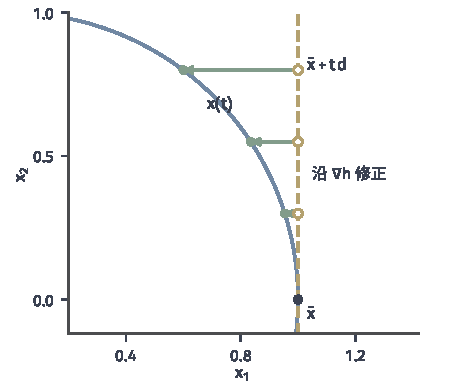
\includegraphics[width=78mm]{figures/05-optimization/06-constrained-optimization/matplotlib/kkt-licq-correction/figure.pdf}
  \caption{用隐函数定理修正线性化方向。蓝线是单位圆周，黄色虚线是切线$\bar{\bm{x}}+t\bm{d}$，黄色空心点是不可行的试探点。绿色箭头沿$\nabla h(\bar{\bm{x}})$方向把试探点拉回圆周，绿点组成可行曲线$\bm{x}(t)$。$t$越小，修正量相对$t$越小。}
  \label{fig:kkt-licq-correction}
\end{BookInlineFigure}

有了可行曲线，线性化方向就全部是真实方向。

\begin{theorem}[LICQ下线性化准确]
\label{thm:kkt-licq-exact}
设约束函数在$\bar{\bm{x}}\in\bm{C}$附近连续可微，$\bar{\bm{x}}$满足LICQ。则
\begin{equation}
 \bm{T}_{\bm{C}}(\bar{\bm{x}})=\bm{F}(\bar{\bm{x}}).
 \label{eq:kkt-licq-exact}
\end{equation}
\end{theorem}

\begin{proof}
包含$\subseteq$是定理~\ref{thm:kkt-tangent-in-linearized}。反过来取$\bm{d}\in\bm{F}(\bar{\bm{x}})$，令
\[
 W=\{i\in A(\bar{\bm{x}}):\langle\nabla g_i(\bar{\bm{x}}),\bm{d}\rangle=0\}.
\]
LICQ保证引理~\ref{lem:kkt-feasible-curve}的线性无关假设成立，得到可行曲线。取$t_k=\delta/(k+1)$，$\bm{x}^{(k)}=\bm{x}(t_k)$，由$\bm{x}'(0)=\bm{d}$知式~\eqref{eq:kkt-tangent-limit}成立，所以$\bm{d}$是切向量。
\end{proof}

\paragraph{条件与约束的写法有关}
LICQ是对约束函数的要求，不是对集合的要求。把预算约束$x_1+x_2\leq\tau$写两遍，可行集一点没变，切锥也没变，但活动梯度$(1,1)$出现两次，线性相关，LICQ就不成立了，见图~\ref{fig:kkt-licq-representation}(b)。这说明LICQ可以因为写法上的冗余而失败，并不代表集合本身有什么毛病。下一小节的条件能容忍这种冗余。

\subsection{Mangasarian--Fromovitz条件}
\label{sec:kkt-mfcq}

回头看证明，线性化准确真正需要什么？对活动不等式来说，严格向内的方向不必拉回，因为它们本来就有一阶余量。只有等式约束要靠拉回来保持。所以只需要等式约束可以被独立修正，并且存在一个同时严格改善所有活动不等式的方向。

\begin{definition}[Mangasarian--Fromovitz约束资格]
\label{def:kkt-mfcq}
设$\bar{\bm{x}}\in\bm{C}$。若$\nabla h_j(\bar{\bm{x}})$（$j=1,\ldots,p$）线性无关，并且存在$\bar{\bm{d}}\in\mathbb{R}^n$，使
\begin{equation}
 \begin{aligned}
  \langle\nabla h_j(\bar{\bm{x}}),\bar{\bm{d}}\rangle&=0,\quad j=1,\ldots,p,\\
  \langle\nabla g_i(\bar{\bm{x}}),\bar{\bm{d}}\rangle&<0,\quad i\in A(\bar{\bm{x}}),
 \end{aligned}
 \label{eq:kkt-mfcq}
\end{equation}
就称$\bar{\bm{x}}$满足\term{Mangasarian--Fromovitz约束资格}（Mangasarian--Fromovitz constraint qualification，MFCQ）。
\end{definition}

条件的两部分各有用途：等式梯度线性无关让我们能用隐函数定理保持等式；方向$\bar{\bm{d}}$让我们能严格走进不等式的内部。图~\ref{fig:kkt-mfcq-direction}(a)中三条活动梯度在平面内必然线性相关，LICQ不成立，但它们都落在某个开半平面内，绿色的$\bar{\bm{d}}$同时与三者成钝角，MFCQ成立。图(b)是尖点：要求$\bar{d}_2<0$与$-\bar{d}_2<0$，两个开半平面不相交，这样的方向不存在。

\begin{BookInlineFigure}
  \centering
  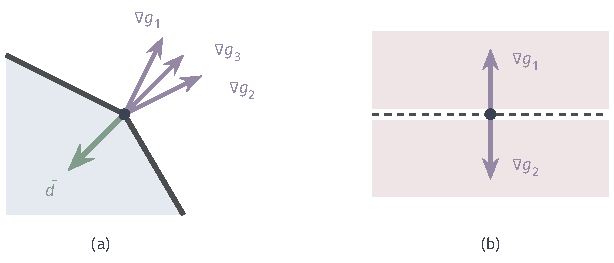
\includegraphics[width=103.9mm]{figures/05-optimization/06-constrained-optimization/tikz/kkt-mfcq-direction/figure.pdf}
  \caption{MFCQ要求存在严格向内的方向。(a)三条活动约束的梯度（紫色）线性相关，但绿色方向$\bar{\bm{d}}$与三者都成钝角，MFCQ成立。(b)两个活动梯度方向相反，使约束严格减小的方向分别在上下两个开半平面（浅红）里，两者不相交，MFCQ不成立。}
  \label{fig:kkt-mfcq-direction}
\end{BookInlineFigure}

两个条件之间有蕴含关系，但不等价。

\begin{lemma}[LICQ蕴含MFCQ]
\label{lem:kkt-licq-implies-mfcq}
若$\bar{\bm{x}}$满足LICQ，则$\bar{\bm{x}}$满足MFCQ。
\end{lemma}

\begin{proof}
以$\nabla h_j(\bar{\bm{x}})$和活动的$\nabla g_i(\bar{\bm{x}})$作行组成矩阵$\bm{J}$，LICQ说明$\bm{J}$行满秩，所以$\bm{J}\bm{J}^\top$可逆。令$\bm{b}$是等式对应分量为$0$、不等式对应分量为$-1$的向量，取
\[
 \bar{\bm{d}}=\bm{J}^\top(\bm{J}\bm{J}^\top)^{-1}\bm{b},
\]
则$\bm{J}\bar{\bm{d}}=\bm{b}$，这正是式~\eqref{eq:kkt-mfcq}。等式梯度作为线性无关组的子集仍线性无关。
\end{proof}

反向不成立。把预算约束写两遍，活动梯度是两个$(1,1)$，LICQ失败；取$\bar{\bm{d}}=(-1,-1)$，内积都是$-2<0$，MFCQ成立。

\begin{theorem}[MFCQ下线性化准确]
\label{thm:kkt-mfcq-exact}
设约束函数在$\bar{\bm{x}}\in\bm{C}$附近连续可微，$\bar{\bm{x}}$满足MFCQ。则式~\eqref{eq:kkt-licq-exact}成立。
\end{theorem}

\begin{proof}
只需证$\bm{F}\subseteq\bm{T}_{\bm{C}}$。取$\bm{d}\in\bm{F}(\bar{\bm{x}})$，对$\epsilon>0$令$\bm{d}_\epsilon=\bm{d}+\epsilon\bar{\bm{d}}$。由式~\eqref{eq:kkt-mfcq}，
\[
 \langle\nabla h_j(\bar{\bm{x}}),\bm{d}_\epsilon\rangle=0,\qquad
 \langle\nabla g_i(\bar{\bm{x}}),\bm{d}_\epsilon\rangle<0,\quad i\in A(\bar{\bm{x}}).
\]

取$W=\varnothing$，引理~\ref{lem:kkt-feasible-curve}的线性无关假设此时只要求等式梯度线性无关，这由MFCQ保证。于是沿$\bm{d}_\epsilon$有可行曲线，$\bm{d}_\epsilon\in\bm{T}_{\bm{C}}(\bar{\bm{x}})$。由引理~\ref{lem:kkt-tangent-closed}，切锥闭，令$\epsilon\downarrow0$得到$\bm{d}\in\bm{T}_{\bm{C}}(\bar{\bm{x}})$。
\end{proof}

这里“先扰动成严格方向，再取极限”这一步是MFCQ证明的关键，它绕开了LICQ需要的全部活动梯度线性无关。

\paragraph{仿射约束与条件的边界}
还有一类不需要任何检查的约束：若全部活动约束和等式约束都是仿射函数，$\bm{d}\in\bm{F}(\bar{\bm{x}})$时直接有$\bar{\bm{x}}+t\bm{d}$在小$t>0$下可行，因此$\bm{T}_{\bm{C}}=\bm{F}$。这正是线性规划不需要讨论约束资格的原因。

约束资格是充分条件，不是线性化准确的必要条件。表~\ref{tab:kkt-three-writings}用同一个集合$\{0\}$的三种写法说明这一点。第三行LICQ和MFCQ都不成立，线性化却是准确的，它属于上面的仿射情形。

\begin{BookInlineTable}
  \centering
  \begin{tabular}{@{}llccc@{}}
    \toprule
    约束写法 & $\bm{F}(0)$ & LICQ & MFCQ & $\bm{T}=\bm{F}$\\
    \midrule
    $x=0$ & $\{0\}$ & 成立 & 成立 & 是\\
    $x^2\leq0$ & $\mathbb{R}$ & 不成立 & 不成立 & 否\\
    $x\leq0$，$-x\leq0$ & $\{0\}$ & 不成立 & 不成立 & 是\\
    \bottomrule
  \end{tabular}
  \caption{同一可行集$\{0\}$的三种写法。切锥恒为$\{0\}$，线性化锥与约束资格随写法改变。}
  \label{tab:kkt-three-writings}
\end{BookInlineTable}

全节的结论可以连成一条链：
\[
 \text{LICQ}\ \Longrightarrow\ \text{MFCQ}\ \Longrightarrow\ \bm{T}_{\bm{C}}=\bm{F}.
\]
有了最后这个等式，切锥上的必要条件就可以放到线性化锥上检验，下一节由此得到关于梯度的方程。
